\documentclass[tikz,border=1.35mm]{standalone}
\usetikzlibrary{arrows.meta}

\definecolor{externalface}{HTML}{8FB9E8}
\definecolor{internalface}{HTML}{F4B46A}
\definecolor{splitred}{HTML}{AF2525}
\definecolor{centroidgreen}{HTML}{0E8814}

% Exploded view of face-based isotropic refinement for a triangular prism.
% The six separated vertex cells duplicate shared edge-midpoint, face-centroid,
% and volume-centroid vertices so each child can be read independently.
\begin{document}
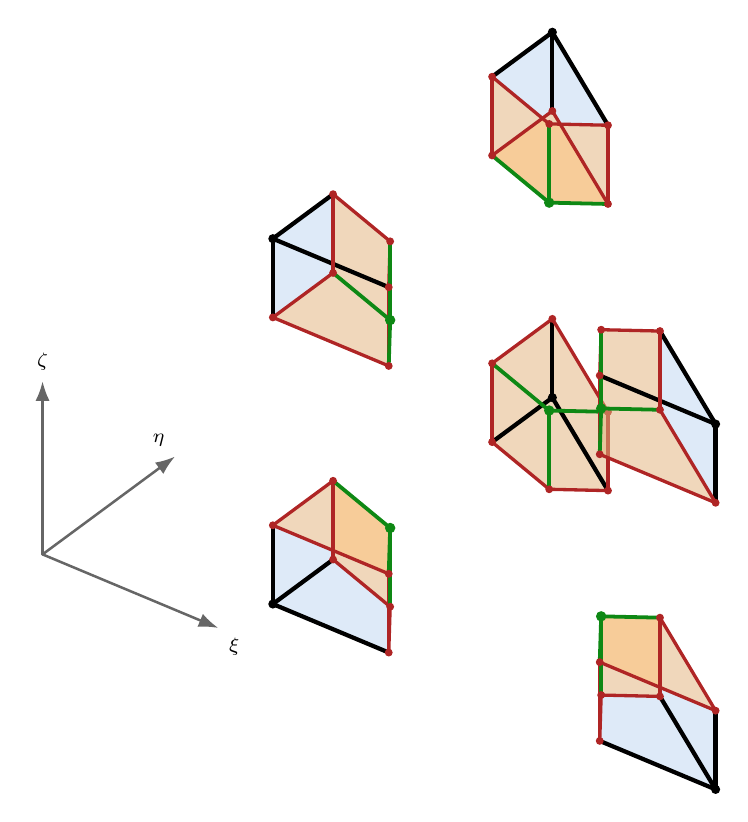
\begin{tikzpicture}[
  x={(20.3mm,-8.5mm)},
  y={(15.3mm,11.3mm)},
  z={(0mm,20mm)},
  line join=round,
  line cap=round,
  outer/.style={draw=black,line width=0.54mm},
  split/.style={draw=splitred,line width=0.42mm},
  centroidedge/.style={draw=centroidgreen,line width=0.48mm},
  cellface/.style={fill=externalface,fill opacity=0.16,draw=none},
  internalcellface/.style={fill=internalface,fill opacity=0.44,draw=none},
  axis/.style={draw=black!60,line width=0.32mm,-{Latex[length=2.5mm,width=1.8mm]}}
]
  \newcommand{\drawcornercell}[8]{%
    \path[cellface] (#1) -- (#2) -- (#5) -- (#3) -- cycle;
    \path[cellface] (#1) -- (#2) -- (#6) -- (#4) -- cycle;
    \path[cellface] (#1) -- (#3) -- (#7) -- (#4) -- cycle;
    \path[internalcellface] (#2) -- (#5) -- (#8) -- (#6) -- cycle;
    \path[internalcellface] (#3) -- (#5) -- (#8) -- (#7) -- cycle;
    \path[internalcellface] (#4) -- (#6) -- (#8) -- (#7) -- cycle;
    \draw[outer] (#1) -- (#2);
    \draw[outer] (#1) -- (#3);
    \draw[outer] (#1) -- (#4);
    \draw[split] (#2) -- (#5);
    \draw[split] (#3) -- (#5);
    \draw[split] (#2) -- (#6);
    \draw[split] (#4) -- (#6);
    \draw[split] (#3) -- (#7);
    \draw[split] (#4) -- (#7);
    \draw[centroidedge] (#5) -- (#8);
    \draw[centroidedge] (#6) -- (#8);
    \draw[centroidedge] (#7) -- (#8);
    \fill[black] (#1) circle[radius=0.58mm];
    \foreach \p in {#2,#3,#4,#5,#6,#7} {
      \fill[splitred] (\p) circle[radius=0.50mm];
    }
    \fill[centroidgreen] (#8) circle[radius=0.66mm];
  }

  % Compact orientation axes, tucked away from the exploded cells.
  \coordinate (Oaxis) at (-1.95,-0.86,-0.78);
  \draw[axis] (Oaxis) -- (-0.85,-0.86,-0.78) node[below right,font=\scriptsize] {$\xi$};
  \draw[axis] (Oaxis) -- (-1.95,0.24,-0.78) node[above left,font=\scriptsize] {$\eta$};
  \draw[axis] (Oaxis) -- (-1.95,-0.86,0.32) node[above,font=\scriptsize] {$\zeta$};

  % Corner A child: edges AB, AC, and AD.
  \begin{scope}[shift={(-0.66,-0.66,-0.66)}]
    \coordinate (O) at (0,0,0);
    \coordinate (X) at (0.725,0,0);
    \coordinate (Y) at (0,0.5,0);
    \coordinate (Z) at (0,0,0.5);
    \coordinate (XY) at (0.483,0.333,0);
    \coordinate (XZ) at (0.725,0,0.5);
    \coordinate (YZ) at (0,0.5,0.5);
    \coordinate (CV) at (0.483,0.333,0.5);
    \drawcornercell{O}{X}{Y}{Z}{XY}{XZ}{YZ}{CV}
  \end{scope}

  % Corner B child: edges BA, BC, and BE.
  \begin{scope}[shift={(0.66,-0.66,-0.66)}]
    \coordinate (O) at (1.45,0,0);
    \coordinate (X) at (0.725,0,0);
    \coordinate (Y) at (0.725,0.5,0);
    \coordinate (Z) at (1.45,0,0.5);
    \coordinate (XY) at (0.483,0.333,0);
    \coordinate (XZ) at (0.725,0,0.5);
    \coordinate (YZ) at (0.725,0.5,0.5);
    \coordinate (CV) at (0.483,0.333,0.5);
    \drawcornercell{O}{X}{Y}{Z}{XY}{XZ}{YZ}{CV}
  \end{scope}

  % Corner C child: edges CB, CA, and CF.
  \begin{scope}[shift={(-0.66,0.66,-0.66)}]
    \coordinate (O) at (0,1,0);
    \coordinate (X) at (0.725,0.5,0);
    \coordinate (Y) at (0,0.5,0);
    \coordinate (Z) at (0,1,0.5);
    \coordinate (XY) at (0.483,0.333,0);
    \coordinate (XZ) at (0.725,0.5,0.5);
    \coordinate (YZ) at (0,0.5,0.5);
    \coordinate (CV) at (0.483,0.333,0.5);
    \drawcornercell{O}{X}{Y}{Z}{XY}{XZ}{YZ}{CV}
  \end{scope}

  % Corner D child: edges DE, DF, and DA.
  \begin{scope}[shift={(-0.66,-0.66,0.66)}]
    \coordinate (O) at (0,0,1);
    \coordinate (X) at (0.725,0,1);
    \coordinate (Y) at (0,0.5,1);
    \coordinate (Z) at (0,0,0.5);
    \coordinate (XY) at (0.483,0.333,1);
    \coordinate (XZ) at (0.725,0,0.5);
    \coordinate (YZ) at (0,0.5,0.5);
    \coordinate (CV) at (0.483,0.333,0.5);
    \drawcornercell{O}{X}{Y}{Z}{XY}{XZ}{YZ}{CV}
  \end{scope}

  % Corner E child: edges ED, EF, and EB.
  \begin{scope}[shift={(0.66,-0.66,0.66)}]
    \coordinate (O) at (1.45,0,1);
    \coordinate (X) at (0.725,0,1);
    \coordinate (Y) at (0.725,0.5,1);
    \coordinate (Z) at (1.45,0,0.5);
    \coordinate (XY) at (0.483,0.333,1);
    \coordinate (XZ) at (0.725,0,0.5);
    \coordinate (YZ) at (0.725,0.5,0.5);
    \coordinate (CV) at (0.483,0.333,0.5);
    \drawcornercell{O}{X}{Y}{Z}{XY}{XZ}{YZ}{CV}
  \end{scope}

  % Corner F child: edges FE, FD, and FC.
  \begin{scope}[shift={(-0.66,0.66,0.66)}]
    \coordinate (O) at (0,1,1);
    \coordinate (X) at (0.725,0.5,1);
    \coordinate (Y) at (0,0.5,1);
    \coordinate (Z) at (0,1,0.5);
    \coordinate (XY) at (0.483,0.333,1);
    \coordinate (XZ) at (0.725,0.5,0.5);
    \coordinate (YZ) at (0,0.5,0.5);
    \coordinate (CV) at (0.483,0.333,0.5);
    \drawcornercell{O}{X}{Y}{Z}{XY}{XZ}{YZ}{CV}
  \end{scope}
\end{tikzpicture}
\end{document}
